\documentclass{jdrp}
\usepackage{lipsum}

\bibliography{example} 

\newcommand*{\crg}{{\aurebesh\Large \$}} % Symbol for Galactic Credits

\begin{document}

    \begin{titlepage}

    \begin{center}
        \hspace*{\vfill}
        \noindent\Huge\jedifont{Star Wars Redemption}\\ 
        \noindent\fontsize{50}{70}\jedifont{\$}
        \noindent\fontsize{50}{70}\jedifont{\#}\\
        \noindent\fontsize{40}{60}\jedifont{Tex Class}
        \hspace*{\vfill}
    \end{center}

    \noindent\makebox[\textwidth]{
        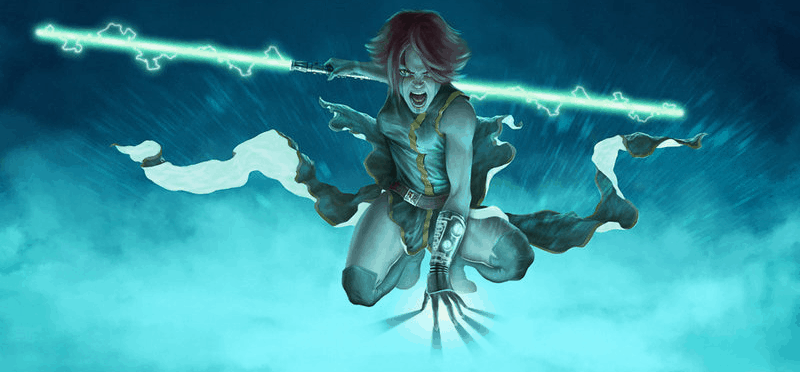
\includegraphics[width=\paperwidth]{_img/cover-bg.png}}
    \end{titlepage}

    \section{Section}

    \lipsum[1]

    \begin{rebelist}
        \item first
        \item second
        \item third
    \end{rebelist}

    \newpage % New column
    \subsection{Sub Section}
    \lipsum[2]

    \begin{quotebox}
        \lipsum[3]
    \end{quotebox}
    
    \begin{enumerate}
        \item first
        \item second
        \item third
    \end{enumerate}

    \clearpage %new page
    \subsubsection{Sub Sub Section}
    \begin{paperbox}{Paperbos}
    You can use special characters as \crg
    \end{paperbox}
    
    \paragraph{Paragraph}
    \lipsum[4]

    \paragraph{Paragraph}
    \lipsum[5]

    \onecolumn
    \nocite{*}
    \printbibliography
\end{document}